\documentclass[14pt]{extarticle}

\usepackage[T1]{fontenc}
\usepackage[utf8]{inputenc}

\usepackage[hidelinks]{hyperref}

\usepackage{microtype}

\usepackage{amssymb}
\usepackage{amsmath}
\usepackage{mathtools}
\usepackage{dsfont}

\usepackage{enumitem}

\usepackage{tikz}
\usetikzlibrary{cd, patterns, patterns.meta, decorations.pathmorphing}

\usepackage{geometry}
\geometry{a4paper, total={170mm, 252mm}, top=22mm}

\usepackage[skip=7pt]{parskip}

\usepackage{graphicx}
\graphicspath{./ilustracje}


\newcommand{\R}{\mathbb{R}}

\def\labelitemi{--}

\usepackage{url}

\usepackage[numbers]{natbib}

\renewcommand{\phi}{\varphi}

\renewcommand{\epsilon}{\varepsilon}

\usepackage{titlesec}
\titlelabel{\thetitle.\quad}

\renewcommand{\contentsname}{Spis treści}
\renewcommand{\bibsection}{\section*{Bibliografia}}

\usepackage{pgfplots}
\pgfplotsset{compat=1.18}


\title{Modelowanie horyzontów zdarzeń czarnych dziur przy użyciu metryki Schwarzschilda: Rozwiązania analityczne i numeryczne}
\author{Aleksandra Niedziela \and Weronika Jakimowicz}
\date{Grudzień 2023}

\begin{document}

\maketitle 
\thispagestyle{empty}
\newpage

\tableofcontents 
\newpage
\setcounter{page}{1}

\section{Wstęp}

\subsection{Czarne dziury Schwarzschilda}

Czarne dziury fascynują i przerażają. Są to obiekty rodem z science fiction - punkt o zerowej objętości i nieskończonej gęstości otoczony tajemniczym horyzontem zdarzeń. Nic dziwnego, że sam Einstein, jak i wielu naukowców, nie mogli uwierzyć w ich istnienie.

Czarne dziury powstają w wybuchu supernowej, kiedy gwieździe skończy się paliwo, a reakcje termojądrowe zatrzymają się, grawitacja zgniata masę do jednego malutkiego punktu - osobliwości. Jego masa jest tak wielka, że zakrzywia czasoprzestrzeń i spowalnia czas, a linia po której przekroczeniu nic, nawet światło, nie jest w stanie uciec, nazywamy horyzontem zdarzeń. 

Czarne dziury były inspiracją dla wielu autorów gatunku science fiction - w filmie \emph{Interstellar} pojawia się Gargantua - obiekt o masie 100 milionów Słońc. Gdy podróżnicy docierają na planetę orbitującą wokół czarnej dziury mówią, iż czas płynie tu wolniej. Zjawisko możemy potwierdzić patrząc na wykres, pokazujący stosunek czasu płynącego normalnie, do czasu w zakrzywionej czasoprzestrzeni.

\renewcommand{\figurename}{Wykres}
\begin{figure}[h]
  \centering
  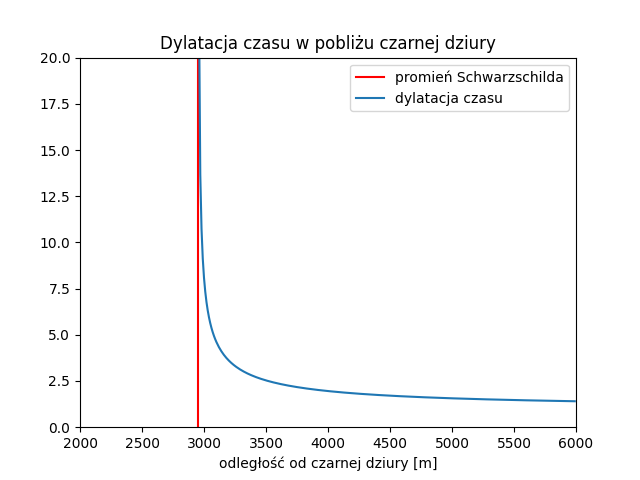
\includegraphics[width=0.7\textwidth]{ilustracje/Time_near_black_hole.png}
  \caption{Stosunek upływu czasu własnego do upływu czasu obserwowanego w punkcie nieskończenie odległym od czarnej dziury w zależności od położenia $r$.}
  %supplement: [Wykres]
%) <time_dilation>
\end{figure}

W 2019 roku otrzymaliśmy pierwsze zdjęcie czarnej dziury, natomiast w maju 2022 roku otrzymaliśmy zdjęcie Saggitariusa A. - jest to supermasywny obiekt w centrum naszej galaktyki \ref{zakazany donut}.

\renewcommand{\figurename}{Zdjęcie}
\begin{figure}[h]
  \centering
  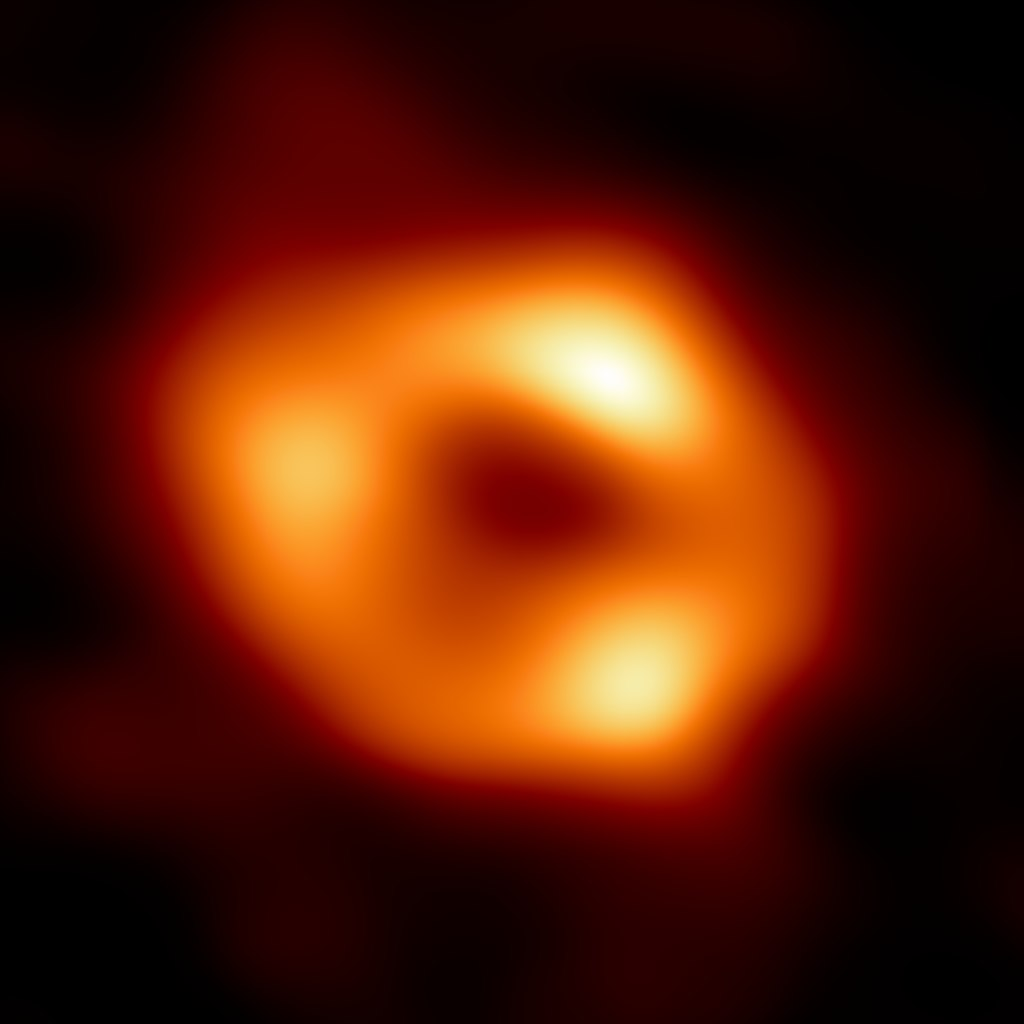
\includegraphics[width=0.7\textwidth]{ilustracje/zakazany_donut.jpg}
  \caption{Zdjęcie czarnej dziury w centrum Mlecznej Drogii uzyskane przez \cite{mleczna_droga}}\label{zakazany donut}
%  supplement: [Figura]
%) <time_dilation>
\end{figure}

Z matematycznego punktu widzenia, czarna dziura jest rozmaitością różniczkowalną z tensorem metrycznym, który opisuje jak zakrzywiona jest przestrzeń wokół niej. Aby więc dokładnie zrozumieć jak zachowują się cząstęczki w jej pobliżu, należy zrozumieć czym są rozmaitości.% i jak wygląda ich geometria.


\subsection{Pojęcie rozmaitości Riemannowskiej}

%Rozmaitości różniczkowalne pozwalają na badanie różnych przestrzeni przez pryzmat przestrzeni $bb(R)^n$. Mówimy, że $M$ jest rozmaitością gładką z atlasem, czyli rodziną map, $cal(A)={ (U_alpha, phi_alpha) }$, jeśli
%- zbiory $U_alpha$ tworzą otwarte pokrycie $M$
%- odwzorowania $phi_alpha:U_alpha arrow overline(U_alpha) subset bb(R)^n$ są homeomorfizmami na otwarte podzbiory $bb(R)^n$, a liczba $n$ jest dobrze określona dla $M$
%- dowolne dwie mapy $(U_alpha, phi_alpha)$ i $(U_beta, phi_beta)$ są *gładko zgodne*, tzn. #list(indent:10pt,
%  [$U_alpha sect U_beta=emptyset$ lub],
%  [mapy przejścia $phi_alpha phi_beta^(-1)$ i $phi_beta phi_alpha^(-1)$ są gładkimi odwzorowaniami pomiędzy podzbiorami $bb(R)^n$.]
%)

Rozmaitość to przestrzeń matematyczna $M$, która wokół każdego punktu $p \in M$ posiada otwarte otoczenie $U_p$, które przypomina pewien podzbiór przestrzeni $\R^n$. Na przykład dla rozmaitości topologicznych owo podobieństwo będzie oznaczało istnienie homeomorfizmu 
$$ \phi_p: U_p \to \overline{U_p} \subseteq \R^n, $$
gdzie $\overline{U_p} \subseteq \R^n$ jest otwartym zbiorem. W niniejszej pracy zajmiemy się opisem czarnej dziury przez Schwarzschilda, który modeluje przestrzeń wokół tej anomalii jako rozmaitość różniczkowalną z tensorem metrycznym, czyli rozmaitość Riemannowską. Dokładna definicja rozmaitości różniczkowalnej znajduje się w dodatku \ref{dodatek rozmaitosci}.


%Dla dowolnego punktu $p in M$ mówimy, że $T_p M$ jest *przestrzenią styczną* w punkcie $p$, czyli przestrzenią zawierającą wektory styczne w tym punkcie. $"TM"$ to z kolei rozłączna suma po wszystkich przestrzeniach stycznych, którą nazywamy *wiązką styczną*. Bardzo ciekawą własnością przestrzeni stycznych jest ich liniowość @leeSmoothManifolds, tzn. dla każdego $p in M$ przestrzeń $T_p M$ jest przestrzenią wektorową wymiaru $n$, a jeśli $(U, phi)$, $phi=(phi_1,...,phi_n)$ jest mapą wokół $p$, to zbiór
%$ { diff phi_1,..., diff phi_n }, $
%gdzie $diff phi_j$ można również oznaczyć $frac(diff, diff phi_j)$, jest bazą $T_p M$.

Przestrzenie styczne w dowolnym $p\in M$ są przestrzeniami wektorowymi oznaczanymi $T_pM$ (dokładna definicja w {dodatku} \ref{dodatek rozmaitosci}). W wielu przypadkach możemy więc zdefiniować na nich iloczyn skalarny, w tym ujęciu nazywany \textbf{tensorem metrycznym} lub też prościej metryką.

Formalnie, tensor metryczny to rodzina dwuliniowych funkcji
$$ g_p:T_p M \times T_p M \to \R $$
zdefiniowana w każdym punkcie $p \in M$. Każda taka funkcja jest dodatnio określonym iloczynem wewnętrznym na $T_p M$, czyli pociąga za sobą normę 
$$ \|v\|_p=\sqrt{g_p (v, v)}. $$
Tensor metryczny określony na $T M$ przypisuje więc dwóm wektorom stycznym $X_p, Y_p$ zaczepionym w punkcie $p$ rozmaitości $M$ wartość
$$ g(X_p, Y_p):= g_p (X_p, Y_p). $$
Ponieważ $g$ jest odwzorowaniem liniowym na $T_p M$ dla każdego $p \in M$, to zapisuje się ono macierzą, którą nazwiemy $g$. Jej wyraz odpowiadający $g(\partial \phi_i, \partial \phi_j)$ będziemy oznaczać $g_{i,j}$.

Warto zaznaczyć, że mając bazę dualną $\{d \phi^i\}$ do $\{ \partial \phi_i\}$, tensor metryczny możemy zapisać jako
$$ g=\sum_{i, j <= n} g_{i, j} d \phi^i \otimes d \phi^j. $$

W tej pracy zajmujemy się metryką Schwarzschilda zdefiniowaną na podzbiorze $\R \times (0, +\infty) \times S^2$ o znakach $(-, +, +, +)$, który jest standardowo zapisywany jako
$$ g = c^2 d \tau^2 = -\frac{r - r_s}{r}\cdot c^2d t^2 + \left( \frac{r - r_s}{r}\right)^{-1} d r^2 + r^2(d \theta^2 + \sin^2(\theta) d \phi^2) $$
lub w postaci macierzy \cite{notatkiUoCSD}
$$
g_{\mu, \nu} = \begin{bmatrix}
  -\frac{1 - r_s}{r}\cdot c^2 & 0                               & 0   & 0 \\
  0                 & \left(\frac{1 - r_s}{r}\right)^{-1} & 0   & 0 \\
  0                 & 0                                   & r^2 & 0 \\ 
  0                 & 0                                   & 0   & r^2 \sin^2(\theta)
\end{bmatrix}, 
$$
gdzie 
\begin{itemize}
  \item $r_s$ to promień Schwarzschilda określonej czarnej dziury, 
  \item $c$ oznacza prędkość światła, 
  \item $\tau$ to czas właściwy (czyli mierzony w pobliżu czarnej dziury), 
  \item $t$ to czas bezwzględny (mierzony nieskończenie daleko od czarnej dziury), 
  \item $\theta$ to kąt po południku, 
  \item a $\phi$ to kąt po równoleżniku.
\end{itemize}




\section{Szybki kurs geometrii}

 \subsection{Proste ścieżki na zakrzywionych powierzchniach - motywacja}

Foton poruszający się w przestrzeni kosmicznej nie jest pod wpływem zewnętrznych sił. Jest cząsteczką, na której prędkość nie wpływają zewnętrzne (ani wewnętrzne) siły, więc jego przyspieszenie przez całą podróż przez czasoprzestrzeń wokół badanej czarnej dziury pozostaje równe $0$. Z drugiej strony, nie posiada on masy, więc nie zachowuje się całkowicie jak cząsteczki materii.

Oznaczmy przez $BH$ rozmaitość opisującą czasoprzestrzeń wokół rozważanej czarnej dziury Schwarzschilda, która zazwyczaj ma postać
$$ BH = \R \times (0,+\infty) \times S^2 $$
Wówczas podróż fotonu jest opisywana przez krzywą
$$ \gamma:I \to BH $$
gdzie $I$ jest pewnym odcinkiem, a nawet może być całą prostą $\R$. Ponieważ foton porusza się z prędkością światła i nie przyspiesza, to wiemy, że
$$\frac{d^2 \gamma} {d t^2}=0.$$ 
Wydaje się, iż dostajemy proste równania różniczkowe opisujące zachowanie funkcji czterowymiarowej.

\renewcommand{\figurename}{Rysunek}
\begin{figure}[h] 
  \centering 
  \vspace{1cm}
  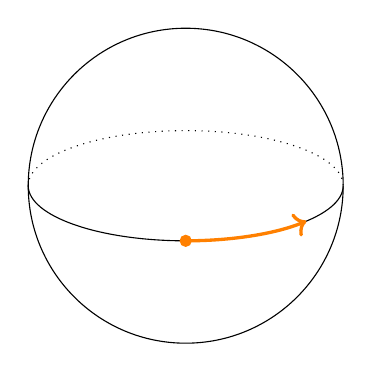
\begin{tikzpicture}
    \draw (0, 0) circle (2);
    \draw (-2, 0) arc (180:360:2 and 0.7);
    \draw[dotted] (-2, 0) arc (180:0:2 and 0.7);

    \draw[very thick, ->, orange] (0, -0.7) arc (270:320:2 and 0.7);
    \filldraw[orange] (0, -0.7) circle (2pt);
  \end{tikzpicture}
  \caption{Cząsteczka poruszająca się po sferze $S^2$.}\label{czasteczka po sferze}
  \vspace{1cm}
\end{figure}

Sprawy nie są jednak tak proste, gdyż metryka zadana na $BH$ mówi nam, że przestrzeń wokół czarnej dziury nie jest do końca taka jak przestrzeń $\R^4$. Jest ona nieco zakrzywiona i to właśnie to zakrzywienie czasoprzestrzeni będzie wpływać na obserwowane przez nas zakrzywienie trasy fotonu w pobliżu czarnej dziury. Aby zrozumieć to lepiej, wyobraźmy sobie, że foton porusza się wzdłuż równika na sferze $S^2$. Wówczas pomimo, że foton nie przyśpiesza w rozumieniu jego podróży po bardzo zagiętej przestrzeni, to dla obserwatora z zewnętrz jego prędkość cały czas się zmienia, jak na rysunku \ref{czasteczka po sferze}.

To zjawisko jest też wyrażone w tym jak różny jest produkt skalarny na badanej przez nas przestrzeni od produktu skalarnego w przestrzeni euklidesowej. Iloczyn metryczny mówi jak długi jest dany wektor, a długość krzywej jest zależna od długości wektorów, które na niej leżą. W takim razie najkrótsza droga między dwoma punktami, czyli droga z zerową drugą pochodną, będzie się zmieniać razem ze zmianą metryki. 

%Stąd nie zawsze prosta droga jest najkrótszą ścieżką między dwoma punktami. Nie jest trudno zauważyć, że tensor metryczny na jednostkowej sferze $S^2$ przedstawia się macierzą
%$$ g_(mu, nu) = \begin{bmatrix}
%  1 & 0\\
%  0 & \sin^2(\theta)\\
%\end{bmatrix} $$
%lub równoważnie wzorem $ds^2 = d \theta^2 + \sin^2(\theta) d \phi^2$, który wynika z wyliczenia długości wektora powstałego zmianę kąta $\phi$ o niewielkie zaburzenie $d \phi$ oraz kąta $\theta$ o niewielkie zaburzenie $d \theta$.
%
%Wiemy już, że pomimo braku przyśpieszenia na zakrzywionej czasoprzestrzeni wokół dziury foton będzie sprawiał wrażenie skręcającego. Chcielibyśmy teraz umieć zrekonstruować jak obserwator w $\R^3$ widzi trasę fotonu w otoczeniu $BH$ mając tylko początkowe położenie i prędkość cząsteczki. 
%


\subsection{Równanie geodezyjnej} %//w pobliżu czarnej dziury Schwarzschilda

%Po pierwsze zauważmy, że nie interesuje nas tak naprawdę samo $gamma$, gdyż ono opisuje tylko położenie w zależności od czasu. W naszym przypadku o wiele bardziej przydatna będzie znajomość wektora prędkości, czyli $frac(d gamma, d t)$, który tak naprawdę jest szczególnym przykładem pola wektorowego wzdłuż krzywej, czyli przyporządkowania 
%$ V:I arrow T"BH" $ 
%takiego, że dla dowolnego $t in I$ zachodzi $V(t) in T_(gamma(t))"BH"$. 
%
%//Rozważmy pokrycie rozmaitości $"BH"$ mapami $(bb(R) times (0, +oo) times U_i^plus.minus, phi_i^plus.minus)$, gdzie zbiory $U_1^+$ i $U_1^-$ to odpowiednio prawa i lewa półkula sfery $S^2$, natomiast $U_2^+$ i $U_2^-$ to górna i dolna półkula. Odwzorowania $phi_i^plus.minus$ to wówczas identyczność na pierwszych dwóch współrzędnych, a rzut na płaszczyznę $bb(R)^2$ z odpowiedniej półkuli. Wiemy, że funkcje $frac(diff, diff (phi_i^plus.minus)^j)$ są bazą przestrzeni stycznej w dowolnym punkcie mapy $phi_i^plus.minus$.]

Ponieważ foton nie przyspiesza podróżując po przestrzeni wokół czarnej dziury, tzn. druga pochodna krzywej opisującej jego trasę jest stale równa zero, to mówimy, że trasa zakreślana przez foton jest \textbf{linią geodezyjną} na rozmaitości $BH$. Linia geodezyjna jest najszybszą (najkrótszą) ścieżką między dwoma punktami - taką właśnie najmniej pochłaniającą energię drogę wybierają zazwyczaj obiekty fizyczne.

Zauważmy, że patrząc na podróż fotonu, przesuwamy wraz z nim przestrzeń styczną, zawierającą wektor prędkości, po krzywej którą ów foton zatacza. Patrząc znów na prosty przykład na $S^2$, przyjrzyjmy się co się dzieje z wektorami stycznymi kiedy przesuwamy je na dwa sposoby między tymi samymi punktami leżącymi na równiku, jak na rysunku \ref{rysunek sfera przestrzenie styczne}.

\begin{figure}[h]
  \centering 
  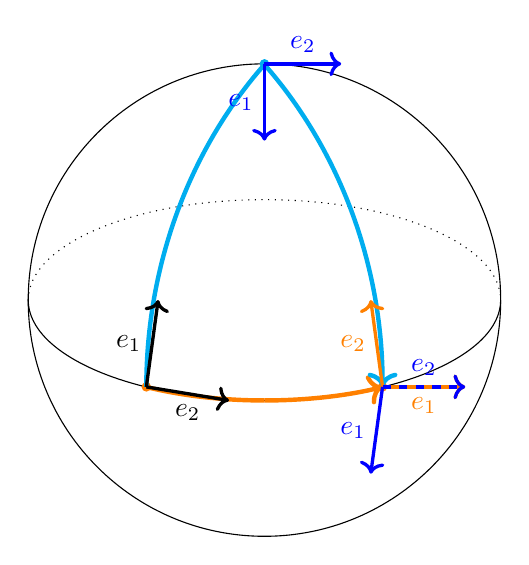
\begin{tikzpicture}
    \draw (0, 0) circle (3);
    \draw (-3, 0) arc (180:360:3 and 1.275);
    \draw[dotted] (-3, 0) arc (180:0:3 and 1.275);

    \draw[orange, ultra thick, ->] (0, -1.275) arc (270:300:3 and 1.275);
    \draw[orange, ultra thick] (0, -1.275) arc(270:240:3 and 1.275);

    \filldraw[orange] (-1.5, -1.1025) circle (1.5pt);
    \filldraw[orange] (1.5, -1.1025) circle (1.5pt);

    \draw[cyan, ultra thick] (-1.5, -1.1025) arc (180:135:5.25 and 5.85);
    \draw[cyan, ultra thick, <-] (1.5, -1.1025) arc (0:45:5.25 and 5.85);

    \filldraw[cyan] (0, 3) circle (1.5pt);

    \draw[->, very thick] (-1.5, -1.1025)--(-1.35, 0) node [midway, left] {$e_1$};
    \draw[->, very thick] (-1.5, -1.1025)--(-0.45, -1.275) node [midway, below] {$e_2$};

    \draw[->, very thick, blue] (0, 3)--(0.975, 3) node [midway, above] {$e_2$};
    \draw[->, very thick, blue] (0, 3)--(0, 2.025) node [midway, left] {$e_1$};

    \draw[->, very thick, orange] (1.5, -1.1025)--(1.35, 0) node [midway, left] {$e_2$};
    \draw[->, very thick, orange] (1.5, -1.1025)--(2.55, -1.1025) node [midway, below] {$e_1$};
    
    \draw[->, very thick, blue, dashed] (1.5, -1.1025)--(2.55, -1.1025) node [midway, above] {$e_2$};
    \draw[->, very thick, blue] (1.5, -1.1025)--(1.35, -2.205) node [midway, left] {$e_1$};
  \end{tikzpicture}
  \caption{Różnica między przestrzeniami stycznymi przesuwanymi po równiku a przestrzeniami stycznymi przesuwanymi po południkach.}\label{rysunek sfera przestrzenie styczne}
\end{figure}

Idąc przez północny biegun sfery wektory styczne obracają się i na końcu trasy nie zgadzają się z wektorami, które były przesuwane po równiku. Przesuwanie wektorów stycznych wzdłuż krzywej kryje w sobie składanie pól wektorowych - pola zawierającego wektory prędkości na krzywej i pola zawierającego wektory bazowe przestrzeni stycznej. W celu uzgodnienia tego, jak przesuwać przestrzeń styczną wzdłuż krzywej, lub bardziej ogólnie jak składać pola wektorowe, potrzebne jest użycie koneksji Levi-Civity, której dokładniejsza definicja znajduje się w dodatku \ref{dodatek koneksja}.

Jeśli teraz $x_1,..., x_n$ są lokalnymi współrzędnymi na rozmaitości, a $\partial_1,...,\partial_n$ wektorami bazowymi przestrzeni stycznej, to możemy zdefiniować \textbf{symbole Christoffela} dla koneksji $\nabla$ względem tego układu współrzędnych jako liczby spełniające poniższą równość:
$$ \nabla_j \partial_k=\Gamma_{j k}^l \partial_l. $$
W przypadku czarnej dziury rolę koneksji Levi-Civity będzie spełniać pochodna względem czasu właściwego $\frac{d}{d\tau}$. W celu uproszczenia notacji i zadowoleniu zmysłu konformizmu z popularną notacją, dla wektora $v$ będziemy pisać 
$$ \nabla v = \frac{d}{d\tau} v = \dot{v}. $$

Niech więc $x_i$ będzie lokalnym układem współrzędnych na $BH$. Wtedy krzywa $\gamma$ zadaje gładkie funkcje $t \mapsto x_i (t)=x_i (\gamma(t))$, które dają funkcję $\R \to \R^4$. W celu uproszczenia notacji będziemy 
od razu pisać $x_i=x_i(t)$. Równanie różniczkowe opisujące geodezyjną którą podróżuje foton przedstawia się wtedy jako
%//$ nabla accent(gamma, dot) (t) = Gamma_(i,j)^k (x_1(t),...,x_4(t))frac(d x^i, d t) frac(d x^j, d t) = 0 $
$$ \ddot{\gamma} = - \Gamma_{i,j}^k \dot{x^i} \dot{x^j} $$
gdzie $\Gamma_{i,j}^k$ to symbol Christoffela drugiego rodzaju \cite{morseTheory}.%//, natomiast $dot$ nad zmienną oznacza branie jej pochodnej względem pewnej affinicznej parametryzacji, która przychodzi razem z koneksją Levi-Civity.

Dodatkowo, ponieważ foton jest cząsteczką bez masy, geodezyjna którą on podróżuje jest określana \emph{nullową} geodezyjną i musi spełniać dodatkowy warunek
$$ g_{\mu,\nu} \dot{x^\mu} \dot{x^\nu} = 0 $$
gdzie $g_{\mu,\nu}$ to wartość tensora metrycznego $g(\mu, \nu)$. Jeśli z kolei zajmowalibyśmy się badaniem cząsteczki z niezerową masą, to wówczas
$$ g_{\mu,\nu} \dot{x^\mu} \dot{x^\nu} = -1\; (\text{patrz \cite{generalRelWald}}). $$




%//wyznaczony za pomocą koneksji Levi-Cevity. W szczególności interesuje nas fakt, że $i$-ta współrzędna wektora prędkości fotonu wyraża się jako
%//$ gamma ^i (t)= -Gamma_(m,j)^i frac(d x^m, d t) gamma ^j (t). $
%
%/*Symbole Christoffela użyte w obliczeniach zostały zaczerpnięte z @symboleGotowe.
%
%Ponieważ foton w naszym przypadku porusza się po płaszczyźnie przechodzącej przez równik, to $x^3 = theta = pi / 2$ jest funkcją stałą. Interesują nas więc tylko wartości zmiany $phi=x^4$ oraz $r=x^2$ w czasie, czyli
%/*$ phi' = -( 1 / r r' phi + 1 / r phi' r)=-( phi / r r' + phi') $
%$ r' = - ( frac(G M, r^2) (1 - (2G M) / r ) t - frac(G M, r^2) (1 - (2G M) / r)^(-1) r' r ) $ */
%
%$ phi' =  -Gamma_(r, phi)^phi r' phi - Gamma_(theta, phi)^phi theta' phi=- frac(r', r) phi - 0 $
%$ r' = -Gamma_(t, t)^r t' t - Gamma_(phi, phi)^r phi' phi -Gamma_(theta, theta)^r theta' theta - Gamma_(r, r)^r r' r = -e^(2 X - 2 V) frac(diff_r X, diff r) t + r e^(-2 V)phi' phi - frac(diff V, diff r) r' r $
%
%gdzie
%$ e^(2x)= e^(-2V)=(1- frac(2G M, c^2 r)) $
%
%Czyli równanie to 
%$ phi' = -frac(r', r) phi $
%$ r' =  $
%*/
%


\section{Matematyczna podróż do czarnej dziury}

W poniższej pracy dokonamy analizy ruchu fotonów w pobliżu czarnej dziury, której promień Schwarzschilda wynosi $r_s=1$. Aby dodatkowo ułatwić rozważania, przyjmujemy $c=G=1$ i konsekwentnie $M=\frac{1}{2}$ oraz ustalamy $\theta=\frac{\pi}{2}$. Dodatkowo, wyliczymy symbole Christoffela drugiego rodzaju dla metryki Schwarzschilda.

\subsection{Symbole Christoffela}

Dla wygody, nie będziemy wyliczać symboli Christoffela wprost z definicji. Zamiast tego, skorzystamy z lagrangianu
%/*Oczywiście, wyliczyć symbole Christoffela można wprost z ich definicji. Prostsze jest jednak użycie lagrangianu, który spełnia*/
$$ S = \int L d \lambda, $$
gdzie $\lambda$ jest afiniczną parametryzacją, a $S$ to działanie, czyli w prostym przypadku cząsteczki poruszającej się wzdłuż pojedynczej krzywej jest to suma iloczynu pędu cząsteczki z fragmentem drogi przebytej \cite{mechanics}. 

%//Używając więc tych faktów w przypadku fotona poruszającego się w metryce Schwarzschilda dostajemy
Stosując więc powyższe wiadomości dla przypadku fotonu poruszającego się w metryce Schwarzschilda dostajemy
$$ S = \int d \tau= \int \frac{d \tau}{d \tau} d \tau = \int \frac{\sqrt{d \tau^2}}{d \tau} d \tau = \int \sqrt{g_{\mu, \nu}\dot{x^\mu} \dot{x^\nu}}d \tau = \int L' d \tau. $$
W takim razie jednym z interesujących nas lagrangianów jest 
$$L'=\sqrt{g_{\mu, \nu}\dot{x^\mu}\dot{x^\nu}}.$$ 
Ponieważ lagrangian nie jest jedyny, i nałożenie na niego dowolnej funkcji dalej daje lagrangian, to możemy wybrać
$$L=(L')^2 = g_{\mu,\nu}\dot{x^\mu}\dot{x^\nu}.$$
Ułatwi to nam wyliczenia korzystające z równań Eulera-Lagrange'a, to znaczy:
$$\frac{d}{ d \tau}\left(\frac{\partial L}{\partial \dot{x^\mu}}\right)= \frac{\partial L}{\partial x^\mu}\; (\text{patrz \cite{mechanics}}). $$
Podstawiając do $d \tau$ metrykę Schwarzschilda dostajemy poniższy układ równań:

\begin{align*}
  \ddot{t}&=-\frac{1}{r(r-1)}\dot{r}\dot{t}\\
  \ddot{r}&=-\frac{r-1}{ 2r^3} \dot{t}^2+\frac{1}{2r(r-1)}\dot{r}^2+(r-1)\dot{\theta}^2+(r-1)\sin^2\theta \dot{\phi}^2\\
  \ddot{\theta} &= \sin \theta \cos \theta \dot{\phi}^2 - \frac{2}{ r} \dot{r}\dot{\theta}\\
  \ddot{\phi} &= -\frac{2}{r} \dot{r}\dot{\phi} - 2 \frac{\cos \theta}{ \sin \theta} \dot{\phi}  \dot{\theta} 
\end{align*}
Zauważmy, że otrzymane wyżej równania to tak naprawdę geodezyjna w metryce Schwarzschilda. Z lewej strony równości można więc z łatwością odczytać symbole Christoffela - są to współczynniki przy odpowiednich pochodnych. Ponieważ interesuje nas tylko ruch fotonów po płaszczyźnie $\theta=\frac{\pi}{2}$, to $\dot{\theta}=0$, $\cos \theta=0$ i $\sin \theta=1$.

Symbole Christoffela w interesującym nas przypadku są więc równe
\begin{align*}
  \Gamma_{t,r}^t&=\frac{1}{2r(r-1)}\\ 
  \Gamma_{t,t}^r&=\frac{r-1}{2r^3}\\ 
  \Gamma_{r,r}^r&=-\frac{1}{2r(r-1)}\\ 
  \Gamma_{\phi,\phi}^r&=-(r-1)\\ 
  \Gamma_{r,\phi}^\phi&=\frac{1}{r} 
\end{align*}

\subsection{Równanie orbity}

Korzystając jeszcze raz z równań Eulera-Langrange'a, dostajemy
$$ \frac{d}{d\tau}(2r^2\dot{\phi})=0 $$
$$ \frac{d}{d\tau}\left(2\frac{r-1}{r}\dot{t}\right)=0 $$
czyli 
$$ r^2\dot{\phi}=a \implies \dot{\phi}=\frac{a}{r^2}$$
$$ \frac{r-1}{r}\dot{t}=\frac{a}{b} \implies \dot{t}=\frac{ra}{b(r-1)}$$
dla pewnych stałych $a,b$. Z fizycznego punktu widzenia $a$ będzie pędem kątowym cząsteczki, natomiast $\frac{a}{b}$ jest energią całkowitą \cite{kolejnaFizyka}. 
%Dzieląc teraz równanie $\dot{t}$ przez równanie $\dot{r}$ uniezależniamy równanie wyżej od czasu właściwego $\tau$.
%$$ \frac{d t}{d\phi}=\frac{br^3}{a(r-1)}$$

%Przekształcając teraz wzór na metrykę Schwarzschilda dostajemy równanie uzależniające $r$ od $\phi$:
%\begin{align*}
%  1&=-\frac{r-1}{r}\dot{t}^2+\frac{r}{r-1}\dot{r}^2+r^2\dot{\phi}^2\\ 
%  \frac{r-1}{r}&=-\frac{(r-1)^2}{r^2}\dot{t}^2+\dot{r}^2+r(r-1)\dot{\phi}^2\\ 
%  %\dot{r}^2&=\frac{r-1}{r}+\frac{(r-1)^2}{r^2}\cdot \frac{a^2r^2}{b^2(r-1)^2}-r(r-1)\frac{a^2}{r^4}\\
%  \dot{r}^2&=\frac{r-1}{r}+\frac{a^2}{b^2}-\frac{a^2(r-1)}{r^3}\\
%  \left(\frac{d r}{d\phi}\right)^2&=\frac{(r-1)r^3}{a^2}+\frac{r^4}{b^2}-r(r-1)\\ 
%  \left(\frac{dr}{d\phi}\right)^2&=\frac{r^4}{b^2}+\frac{r-1}{r}\left(\frac{r^4}{a^2}-r^2\right)
%\end{align*}
%Jak już zostało wspomniane, 
%$$r^2\dot{\phi}^2=a=\frac{L}{\mu},$$
%gdzie $\mu$ to zredukowana masa układu, wynosząca
%$$\mu=\frac{mM}{m+M}=0,$$
%bo $M=1$, ale $m=0$ jako masa fotonu. W takim razie $a\to \infty$ jeśli będziemy zmniejszać masę cząsteczki do $0$. Dla pozostawienia $b$ jako stałej bez wyrazu $r$, wykonamy podstawienie
%$$\begin{matrix}u=\frac{1}{r}\\ -r^2du=dr\end{matrix}$$
%otrzymując ostatecznie równanie orbity
%$$\left(\frac{du}{d\phi}\right)^2=\frac{1}{b^2}+(1-u)\left(\frac{1}{a^2}-u^2\right)\xrightarrow{a\to\infty}\frac{1}{b^2}-u^2(1-u)$$
%które możemy obustronnie zróżniczkować względem $\phi$ by otrzymać
%$$2u''u'=3u^2\cdot u'-2u\cdot u'$$
%$$u''=u\left(\frac{3}{2}u-1\right)$$
%z czego od razu widać, że orbitą stałą jest 
%$$u=\frac{2}{3}\implies r=\frac{3}{2}$$
%

Możemy teraz wyznaczyć $t$ w zależności od $\phi$, pozbywając się zależności od $\tau$:
$$\frac{dt}{d\phi}=\frac{r^3}{b(r-1)}$$
Przekształcając teraz drugi warunek geodezyjnej \emph{nullowej}, dostajemy
\begin{align*}
  0&=-\frac{(r-1)^2}{r^2}(dt)^2+(dr)^2+r(r-1)(d\phi)^2\\ 
  (dr)^2&=\frac{(r-1)^2}{r^2}(dt)^2-r(r-1)(d\phi)^2\\ 
  \left(\frac{dr}{d\phi}\right)^2&=\frac{(r-1)^2}{r^2}\left(\frac{dt}{d\phi}\right)^2-r(r-1)\\ 
  \left(\frac{dr}{d\phi}\right)^2&=\frac{(r-1)^2}{r^2}\cdot\frac{r^6}{b^2(r-1)^2}-r(r-1)\\ 
  \left(\frac{dr}{d\phi}\right)^2&=\frac{r^4}{b^2}-r(r-1)
\end{align*}
a stosując podstawienie 
$$u=\frac{1}{r},\quad -r^2du=dr$$
wyraz $\frac{1}{b^2}$ stanie się wyrazem wolnym, znikającym po różniczkowaniu względem $\phi$:
\begin{align}
  \left(\frac{du}{d\phi}\right)^2&=\frac{1}{b^2}-u^2+u^3\label{rownanie_orbity}\\ 
  u'' &=u\left(\frac{3}{2}u-1\right)\label{zmiana predkosci}
\end{align}

\renewcommand{\figurename}{Wykres}
\begin{figure}[h]
  \centering
  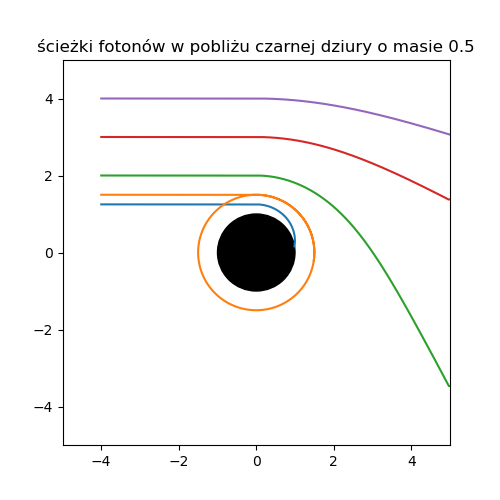
\includegraphics[width=0.8\textwidth]{ilustracje/sceizki_wykres.png}
  \caption{Ścieżki fotonów w pobliżu czarnej dziury o masie $M=\frac{1}{2}$ i promieniu Schwarzschilda $r_s=1$ ($c=1=G$) uzyskane przy pomocy języka Python.}\label{wykres fotonow}
\end{figure}

Powyższe równanie (\ref{zmiana predkosci}) w jasny sposób pokazuje, że orbita stacjonarna w przypadku czarnej dziury o promieniu Schwarzschilda $1$ pojawia się dla $r=\frac{3}{2}$. Wspomniana orbita została zaznaczona na wykresie \ref{wykres fotonow}, który prezentuje również rozmiar czarnej dziury (czarne koło pośrodku). Równanie (\ref{zmiana predkosci}) zostało rozwiązane przy pomocy funkcji \verb+odeint+ z biblioteki \verb+scipy+ języka Python i trajektorie pięciu fotonów, z czego część nie zapada się w czarną dziurę, zostały pokazane na wykresie \ref{wykres fotonow}





%/* 
%Oczywiście, $accent(r, diaer)=0$, bo foton nie przyśpiesza. Możemy więc podzielić drugie równanie przez $accent(phi, dot)^2$, by dostać:
%
%$ 0=frac(r-1, 2r^3)(frac(accent(t, dot), accent(phi, dot)))^2 +frac(1, 2r(r-1))(frac(accent(r, dot), accent(phi, dot)))^2 - (r-1) $
%$ (frac(accent(r, dot), accent(phi, dot)))^2=2r(r-1)^2-frac((r-1)^2, r^2)(frac(accent(t, dot), accent(phi, dot)))^2. $
%
%*/
%
%Chcemy teraz wydobyć $\dot{t}$ oraz $\dot{\phi}$ - wtedy będziemy wiedzieli jak wyrazić $\frac{\dot{t}}{\dot{\phi}}$. Wracając do drugiej równości lagrangiana wykorzystanej dla $phi$ oraz $t$, dostaniemy:
%$ 
%  frac(d, d tau) (2r^2 accent(phi, dot))&=0\ 
%    frac(d, d tau) (2frac(r-1, r)accent(t, dot))&=0
%$
%Co znaczy, że
%$ r^2 accent(phi, dot)=a => accent(phi, dot)=frac(a, r^2) $
%$ frac(r-1, r)accent(t, dot)=frac(a, b) => accent(t, dot) = frac(a r, b(r-1)) $
%dla pewnych stałych $a, b$.
%
%Przekształcając teraz metrykę Schwarzschilda, dostajemy
%$ frac(r-1, r) = frac((r-1)^2, r^2)accent(t, dot)^2 - accent(r, dot)^2 -r(r-1) accent(phi, dot)^2 $
%a podstawiając wartości $accent(phi, dot)^2$ i $accent(t, dot)^2$ wyliczone wyżej
%$ frac(r-1, r) = frac(a^2, b^2) - accent(r, dot)^2 - r(r-1)a^2 $
%$ accent(r, dot)^2 = frac(a^2, b^2) - frac(r-1, r)(1 + frac(a^2, r^2)). $
%Aby teraz wyliczyć równanie orbity, chcemy podzielić powyższe równanie przez $accent(phi, dot)^2=frac(a, r^2)$:
%$ ( frac(accent(r, dot), accent(phi, dot)) )^2 = frac(r^4, b^2) - frac((r-1), r)(frac(r^4, a^2)+r^2) $
%Trzeba tutaj zaznaczyć, że równanie wyliczone wyżej nie jest jeszcze krzywą geodezyjną po której podróżuje światlo - w przypadku wyżej wzięliśmy
%$ -1 = g_(mu, nu)accent(x^mu, dot)accent(x^nu, dot) $
%zamiast przyrównywać to do zera. Badamy więc chwilowo trasę cząsteczki z masą. Aby przejść do badania fotonu, chcemy aby $a arrow oo$. Fizycznie wartość ta jest tak naprawdę równa pędowi kątowemu $L$ wydzielonemu przez zredukowaną masę $mu$, tzn.
%$ r^2 accent(phi, dot)^2 = a = frac(L, mu) $
%a ponieważ zredukowana masa jest zależna od masy fotonu $m_1=0$, 
%$ mu = frac(m_1 m_2, m_1 + m_2), $
%gdzie $m_1, m_2$ to masy składowe układu dwóch ciał, to dla fotonu $mu=0$ i co za tym idzie, $a arrow oo$.
%
%\subsection{Równanie orbity}
%
%W równaniu orbity wyliczonym w poprzednim rozdziale zastosujemy podstawienie $u=frac(1, r)$, wtedy
%$ -r^2 accent(u, dot) = accent(r, dot). $
%Po takim podstawieniu równanie orbity to
%$ ( frac(accent(u, dot), accent(phi, dot)) )^2 = frac(1, b^2) - (1-u)(frac(1, a^2)+u^2) = frac(1, b^2)-(1-u)u^2 $
%bo jak wcześniej uzasadniliśmy, $a arrow oo$.
%
%Rozwiązanie powyższego równania dałoby zależność między $r$ a $phi$, bo możemy usunąć trzymaną z tyłu głowy informację o $tau$:
%$ (frac(d u, d phi))^2 = frac(1, b^2) -(1-u)u^2. $
%Bez trudu wyciągniemy też informację o drugiej pochodnej $u$:
%$ 2u'(phi)u''(phi) = -2u + 3u^2 $
%$ u''(phi) = -u + frac(3, 2) u^2=u(frac(3, 2)u-1), $
%bo $u'=c=1$ w naszym układzie. Stąd widać, że $u=0$ oraz 
%$ frac(2, 3)=u=frac(1, r) => r = frac(3, 2) $ 
%są punktami przegięcia funkcji $u(phi)$. Dalej, dla 
%$ frac(2, 3)< u = frac(1, r) => r < frac(3, 2) $ 
%pochodna $u'(phi)$ powinna być rosnąca (czyli $r'=-r^2u'$ maleje), a dla 
%$ frac(2, 3) > u=frac(1, r) => r > frac(3, 2) $ 
%powinna być malejąca ($r'=-r^2u'$ rośnie).
%
%Możemy więc obserwować pierwiastki powyższej równości, by sprawdzać, kiedy $r(phi)$ jest stałe. Co więcej, możemy również sprawdzić przy jakim położeniu foton zapadnie się w czarną dziurę, a kiedy będzie w stanie uciec z jej pobliża.
%
%Równanie wyżej jest równaniem 3 stopnia o rzeczywistych współczynnikach, ma więc ono 3 pierwiastki, co najmniej jeden rzeczywisty i dwa potencjalnie zespolone, sprzężone ze sobą. Możemy oznaczyć je przez $u_1, u_2, u_3$ i zapisać
%$ 
%  (frac(d u, d phi))^2 &= (u- u_1) (u- u_2) (u-u_3)= \
%    &= u^3 - u^2 (u_1 + u_2 + u_3)+ \ 
%      &+ u(u_1 u_2 + u_1 u_3 + u_2 u_3) +\ 
%        &-u_1 u_2 u_3. 
%$
%
%Widzimy więc, że suma pierwiastków odpowiada wyrazowi przy $u^2$ w oryginalnym równaniu, natomiast ich iloczyn jest równy wyrazowi wolnemu:
%$ 
%  u_1 + u_2 + u_3 = 1
%$
%$
%  -frac(1, b^2) = u_1 u_2 u_3
%$
%%/* 
%%Warto też zauważyć, że oryginalne równanie nie posiada wyrazu stopnia $1$, czyli 
%%$ 0= u_1 u_2 + u_1 u_3 + u_2 u_3 $
%%*/
%
%Z tego wzoru możemy od razu wyliczyć wzór na drugą pochodną
%$ (u'(phi))^2 = (u-u_1)(u-u_2)(u-u_3) $
%$ u''(phi)u'(phi) = frac(1, 2)[(u-u_2)(u-u_3) + (u-u_1)(u-u_2) + (u-u_1)(u-u_3)] $
%gdzie możemy sprawdzać jej wartość w punktach ekstremalnych funkcji $u(phi)$.
%
%Zacznijmy od przypadku gdy $u_1 < u_2 < u_3$ są wszystkie liczbami rzeczywistymi. Wtedy dla $u_2 < u < u_3$ oraz $u < u_1$ funkcja $(u-u_1) (u-u_2) (u-u_3)$ jest ujemna, co daje zespoloną wartość dla $u'(phi)$. 
%
%Jeśli teraz $u_1$ będzie jedynym pierwiastkiem rzeczywistym, a $u_2$ i $u_3$ będą sprzężonymi ze sobą pierwiastkami zespolonymi. W takim przypadku jedyny pierwiastek rzeczywisty musi być ujemny, bo wtedy
%$ -frac(1, b^2) = u_1 u_2 u_3 = u_1 u_2 overline(u_2) = u_1 ("Re"(u_2)^2 + "Im"(u_2)^2) $
%gdzie $b^2$ oraz $"Re"(u_2)^2+"Im"(u_2)^2$ są zawsze dodatnimi wartościami.
%
%W takim razie $u_1$ będzie orbitą, z której fotony nie zapadają się, ale też nie mają szansy wypaść z okolic czarnej dziury. Z racji tego jak wyglądają czarne dziury, możemy z dużą dozą prawdy stwierdzić, że 
%$ u_1>r_s=1. $ 
%W takim razie $"Re"(u_2)="Re"(u_3)<0$.
%
 
%
%= Wyniki symulacji
%
%#include"05_jakie_algorytmy.typ"
%
%= Dodatek
%
%#include"10_dodatek_rozmaitosci.typ"

\section{Dodatek}

\subsection{O rozmaitościach różniczkowalnych}\label{dodatek rozmaitosci}

Rozmaitości różniczkowalne pozwalają na badanie różnych przestrzeni przez pryzmat przestrzeni $\R^n$. Mówimy, że $M$ jest rozmaitością gładką (różniczkowalną) z atlasem, czyli rodziną map, $\mathcal{A}=\{ (U_\alpha, \phi_\alpha) \}$, jeśli
\begin{itemize}
  \item zbiory $U_\alpha$ tworzą otwarte pokrycie $M$
  \item odwzorowania $\phi_\alpha:U_\alpha \to \overline{U_\alpha} \subseteq \R^n$ są homeomorfizmami na otwarte podzbiory $\R^n$, a liczba $n$ jest dobrze określona dla $M$
  \item dowolne dwie mapy $(U_\alpha, \phi_\alpha)$ i $(U_\beta, \phi_\beta)$ są \emph{gładko zgodne}, tzn.
    \begin{itemize}
      \item $U_\alpha \cap U_\beta=\emptyset$ lub
      \item mapy przejścia $\phi_\alpha \phi_\beta^{-1}$ i $\phi_\beta \phi_\alpha^{-1}$ są gładkimi odwzorowaniami pomiędzy podzbiorami $\R^n$.
    \end{itemize}
\end{itemize}

Dla dowolnego punktu $p \in M$ mówimy, że $T_p M$ jest \emph{przestrzenią styczną} w punkcie $p$, czyli przestrzenią zawierającą wektory styczne w tym punkcie. Definiować wektory styczne zaczynamy od zdefiniowania zbioru krzywych zaczepionych w punkcie $p \in M$, czyli zbioru par krzywych $c: (-\varepsilon, \varepsilon) \to M$ i liczb $t_0 \in (-\varepsilon, \varepsilon)$ takich, że $c(t_0)=p$. Jeśli $(U, \phi)$ jest mapą wokół $p \in M$, to definiujemy na zbiorze krzywych zaczepionych w $p$ relację równoważności 
$$ [c_0, t_0] \sim [c_1, t_1] \iff (\phi_p \circ  c_0)'(t_0)=(\phi_p \circ  c_1)'(t_1). $$
Klasy równoważności par $[c, t_0]$ to właśnie wektory styczne należące do $T_p M$.


$T M$ to z kolei rozłączna suma po wszystkich przestrzeniach stycznych, którą nazywamy \emph{wiązką styczną}. Bardzo ciekawą własnością przestrzeni stycznych jest ich liniowość \cite{leeSmoothManifolds}, tzn. dla każdego $p \in M$ przestrzeń $T_p M$ jest przestrzenią wektorową wymiaru $n$, a jeśli $(U, \phi)$, $\phi=(\phi_1,...,\phi_n)$ jest mapą wokół $p$, to zbiór
$$ { \partial \phi_1,..., \partial \phi_n }, $$
gdzie $\partial \phi_j$ można również oznaczyć $\frac{\partial}{\partial \phi_j}$, jest bazą $T_p M$.

Pole wektorowe to z kolei funkcja $X:M\to TM$ taka, że $X(p)\in T_pM$. Często zapisujemy $X(p)=X_p$. Jeśli teraz $c:I\to M$ jest krzywą na rozmaitości $M$, to mówimy, że pole $X$ jest funkcją gładką $X:I\to TM$ taką, że $X(t)\in T_{c(t)}M$ dla każdego $t\in I$.

\subsection{Koneksja Levi-Civity}
\label{dodatek koneksja}

Koneksja Levi-Civity jest definiowana jako pewien rodzaj połączenia affinicznego. Zacznijmy więc od zdefiniowania, czym takie połączenie jest. 

Jeśli $M$ jest rozmaitością gładką, a $X$, $Y$ oraz $Z$ są gładkimi polami wektorowymi na niej, to definiujemy połączenie affiniczne jako pole wektorowe $\nabla_XY$, które dla dowolnego punktu $p\in M$ spełnia
$$(\nabla_XY)_p=\nabla_{X_p}Y,$$
gdzie napis po prawej stronie oznacza przypisanie wektorowi stycznemu $X_p$ oraz polu wektorowemu nowego wektora stycznego $\nabla_{X_p}Y$. Wymagamy, aby wspomniane przypisanie
\begin{itemize}
  \item było dwuliniowe jako funkcja $X_p$ i $Y$ w obrębie przestrzeni stycznej $T_pM$, tzn:
    \begin{itemize}
      \item $\nabla_{X_p+Y_p}Z=\nabla_{X_p}Z+\nabla_{Y_p}Z$
      \item $\nabla_{X_p}(Y+Z)=\nabla_{X_p}Y+\nabla_{X_p}Z$.
    \end{itemize}
  \item dla dowolnej gładkiej funkcji $f:M\to\R$ i pola wektorowego, które przez nią powstaje $(fY)_q=f(q)Y$, spełniało równość
    $$\nabla_{X_p}(fY)=(X_pf)Y_p+\nabla_{f(p)X_p}Y,$$
    gdzie $X_pf$ oznacza pochodną kierunkową $f$ w kierunku $X_p$: jeśli $X_p=[c, t_0]$, to $X_pf:=[f\circ c, t_0]$ \cite{morseTheory}.
\end{itemize}

%Niech teraz $M$ będzie rozmaitością gładką wyposażoną w połączenie affiniczne $\nabla$, a $c:I\to M$ niech będzie krzywą na tej rozmaitości parametryzowaną przez zmienną $t$. Wówczas jeśli $X$ jest polem wektorowym wzdłuż tej krzywej, to istnieje jedyne odwzorowanie między $X$ a polem wektorowym $\frac{DX}{dt}$ takie, że $\frac{D}{dt}$ jest liniowe względem $X$. Jeśli istnieje inne pole wektorowe $Y$ takie, że $X(t)=Y(c(t))$, to wówczas \cite{riemannianCarmo}
%$$\frac{DX}{dt}=\nabla_{\frac{dc}{dt}}Y$$

Niech teraz $M$ będzie rozmaitością riemannowską wyposażoną w tensor metryczny $g$. Wówczas połączenie affiniczne $\nabla$ jest zgodne z metryką wtedy i tylko wtedy gdy dla gładkich pól wektorowych $X,Y,Z$ spełniona jest równość
$$Xg(Y, Z)=g(\nabla_XY, Z)+g(Y, \nabla_XZ)\; (\text{patrz \cite{riemannianCarmo}}).$$

Na każdej rozmaitości riemannowskiej istnieje jedyne połączenie affiniczne $\nabla$, które 
\begin{itemize}
  \item jest zgodne z metryką
  \item oraz jest symetryczne, tzn. dla dowolnych pól wektorowych $X, Y$ mamy 
    $$\nabla_X Y-\nabla_Y X=[X, Y],$$ 
    gdzie $[X, Y]=XY-YX$ jest pochodną Liego $X, Y$ \cite{riemannianCarmo}.
\end{itemize}
Takie połączenie affiniczne $\nabla$ jest nazywane \textbf{koneksją Levi-Civity}.



\bibliographystyle{ACM-Reference-Format}
\bibliography{literatura}

\end{document} 
